\chapter{Forecasting the daily electricity consumption}
\label{cha:Forecasting the daily electricity consumption}
In this chapter the different forecasting techniques to perform a 24 hour prediction for an individual household are discussed. One daily prediction has a data granularity of an half hour, which means that $ 48 $ data points have to be estimated for each prediction. \\\textbf{update --> discussing data}
First pre-processing is done in Section \ref{s:Pre-processing} and the time series used are discussed. Afterwards the baseline models are looked into in Section \ref{s:Baseline models}. These models are characterised by a low calculation load during training and they therefore serve as an easy to obtain result where a more complex model can be compared with. Next, more complex models based on a neural network philosophy are discussed in Section \ref{s:Neural network models}. ``Long Short-Term Memory'' and ``Gated Recurrent Unit'' are most suitable to process time series and therefore serve as the core model which is analysed with different design choices. Finally, a parameter search is conducted. Here, an analysis is made of the sensitivity of the choice of different parameters is made.\\
 
\section{Pre-processing}\label{s:Pre-processing}
The data that is available is summarized by Table \ref{tab:available_data}. 

\subsection{Data}
In order to reduce the calculation load to do the parameter search in Section \ref{s: Parameter search}, three series are selected from the \textit{consumption.csv} that is listed in Table \ref{tab:availablef_data}. The series are chosen based on the least missing values of the historic electrical consumption serie and the absence of a big shift. Figure \ref{fig:three_series} shows the three figures and Table \ref{tab:three_series} summarizes their characteristics.\\

\begin{figure}[ht]
	\begin{subfigure}{0.32\textwidth}
		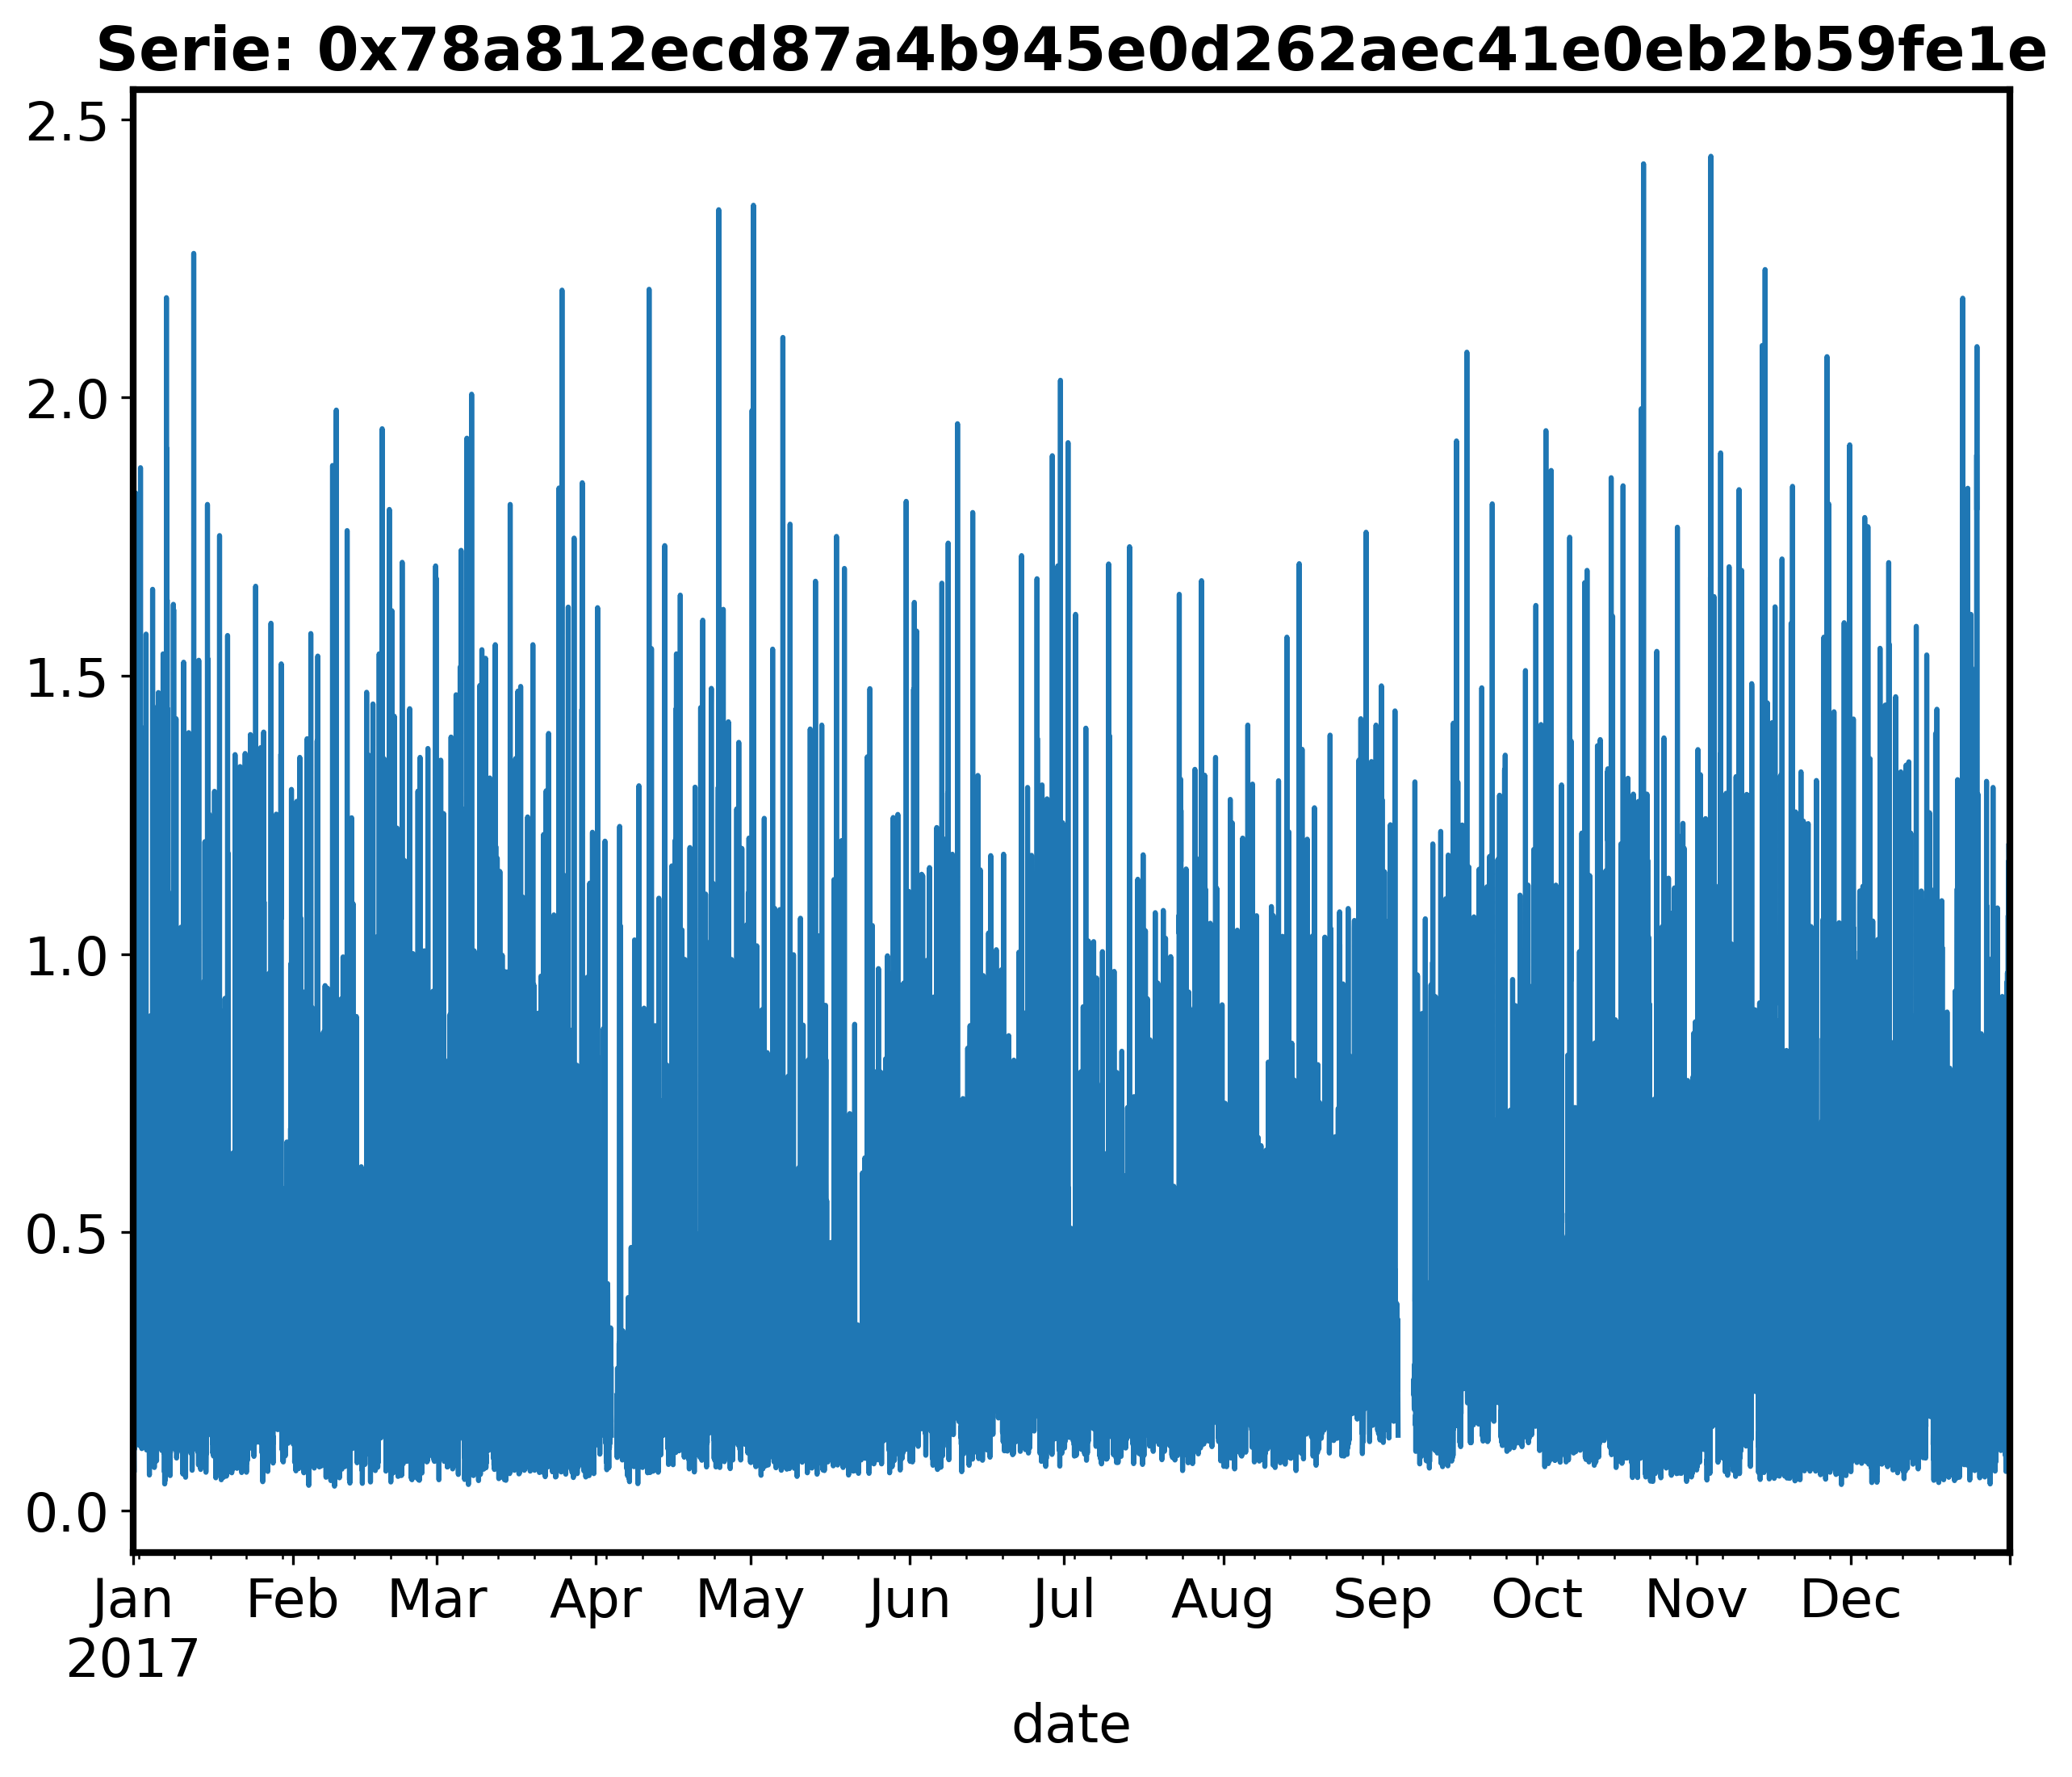
\includegraphics[width=1\linewidth]{Serie0x78a812ecd87a4b945e0d262aec41e0eb2b59fe1e.png}
		\caption{Serie $ 1 $}
	\end{subfigure}	 	
	\begin{subfigure}{0.32\textwidth}
		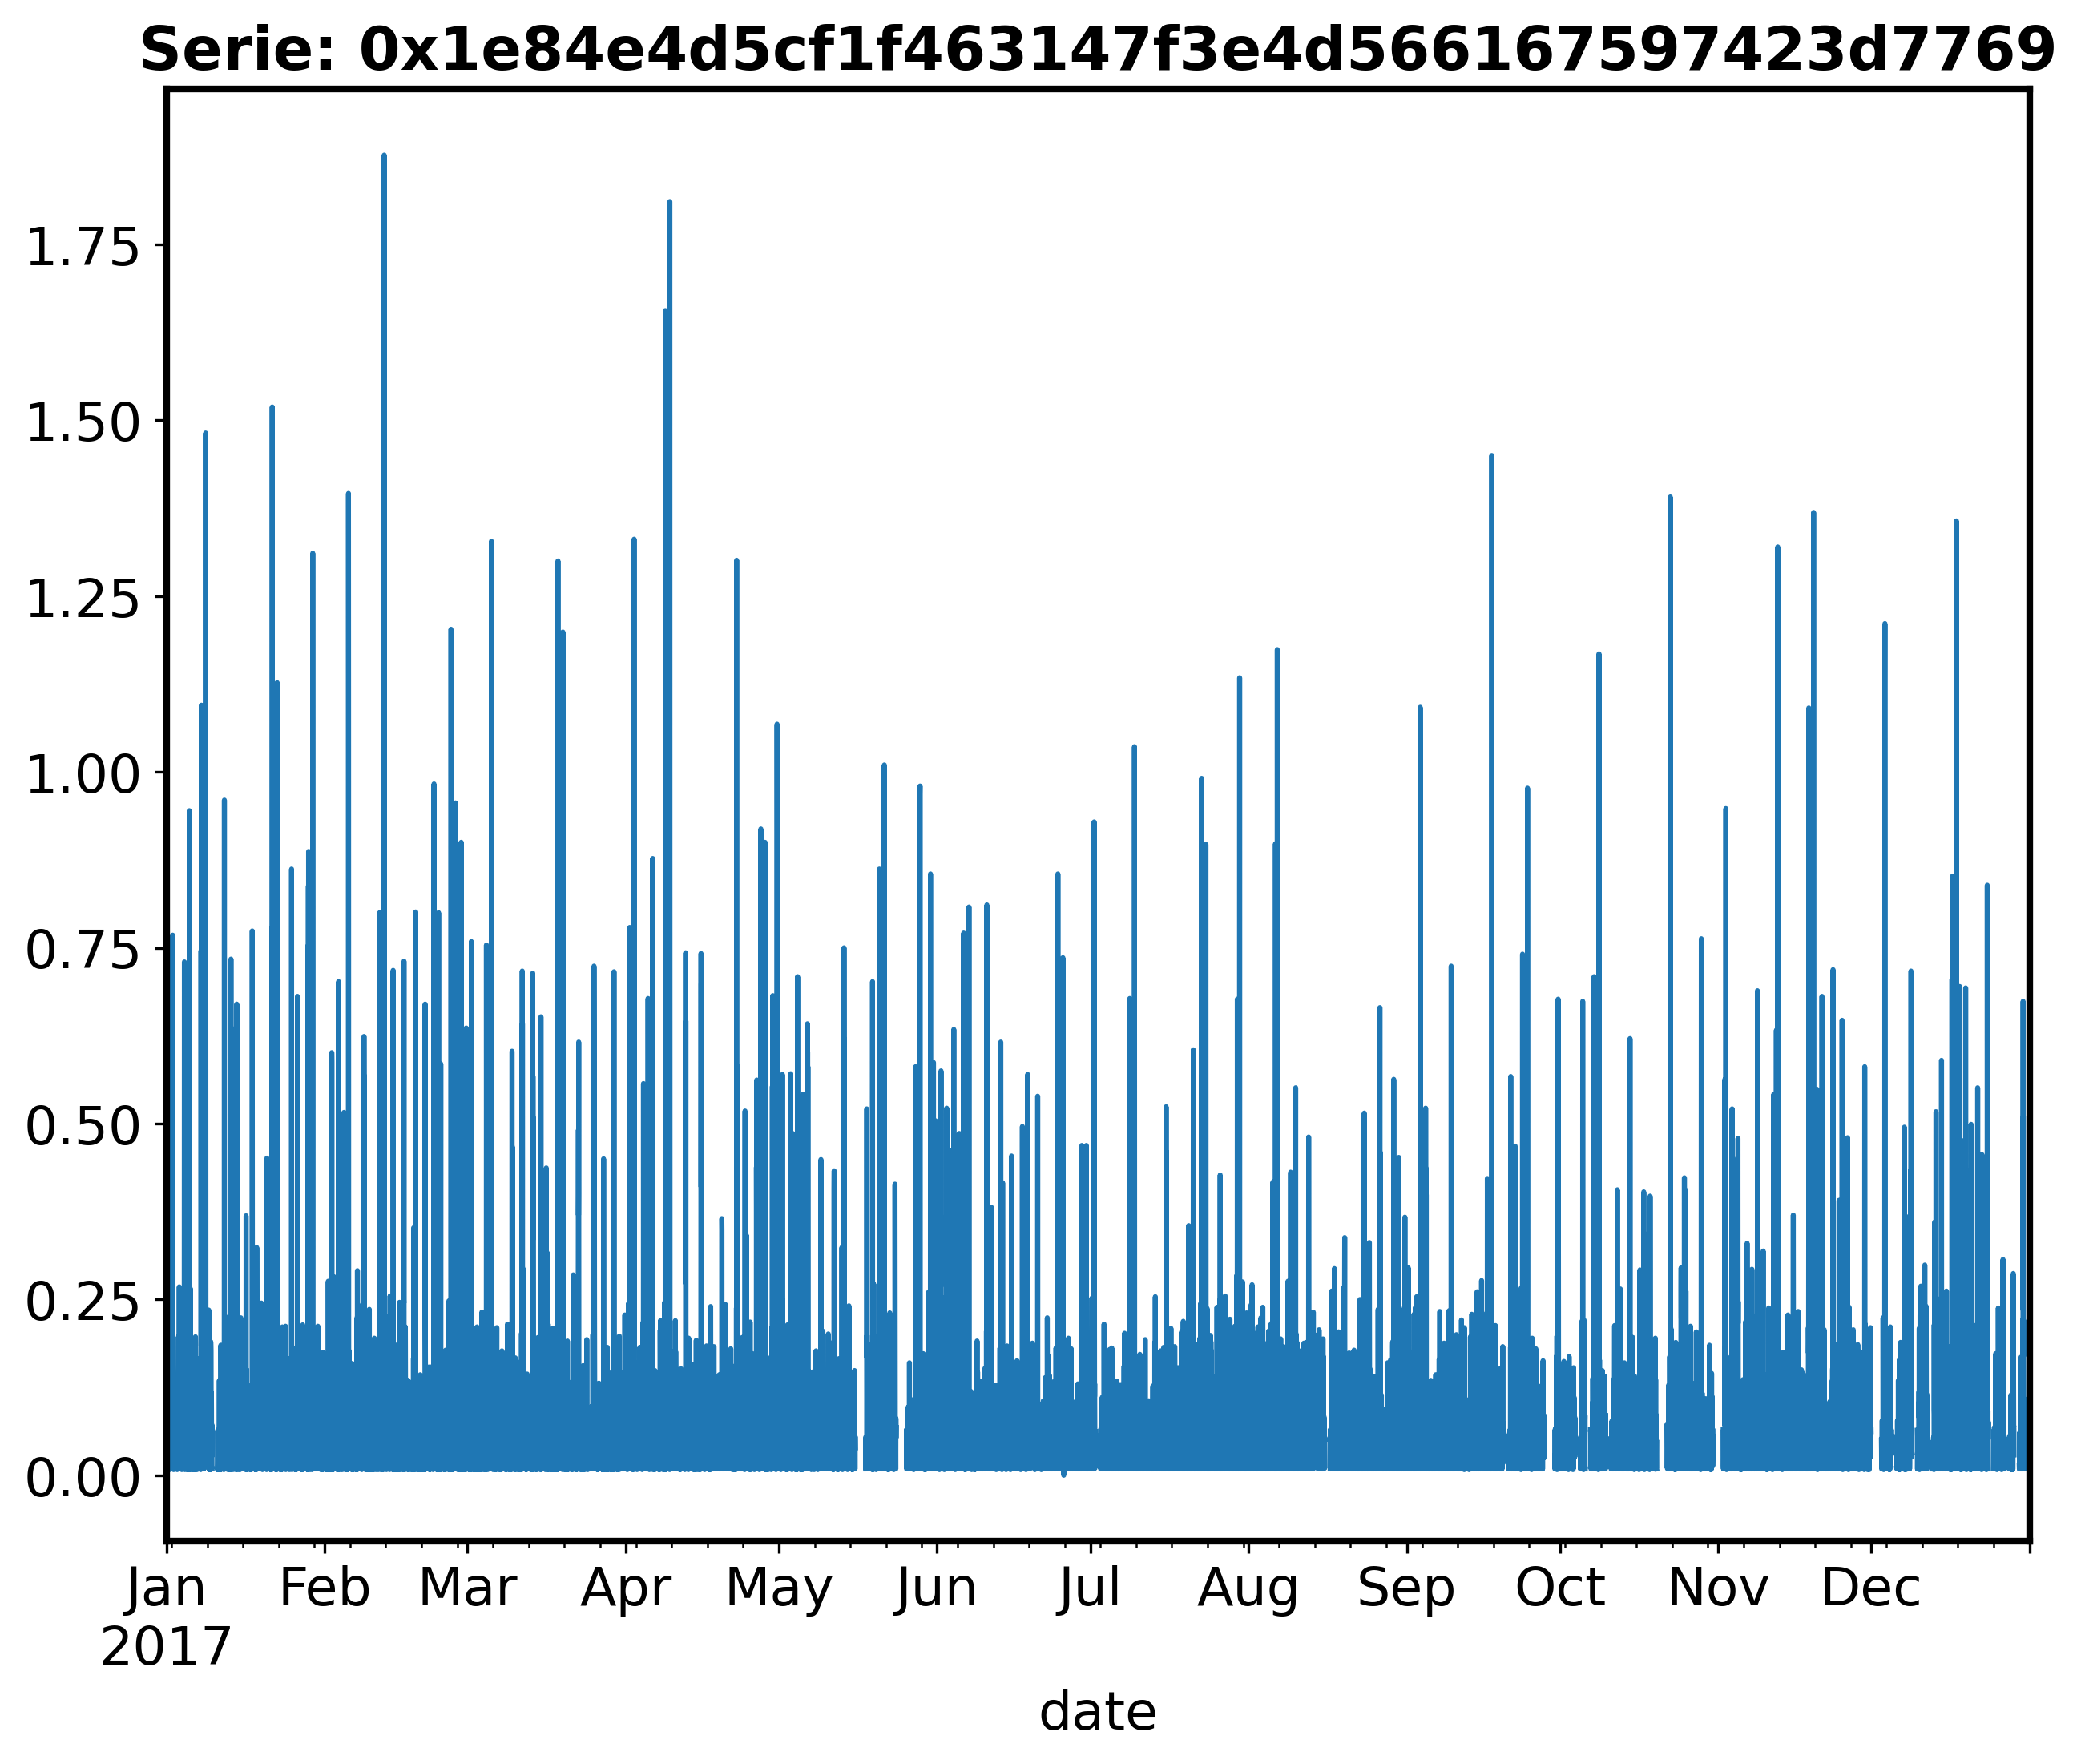
\includegraphics[width=1\linewidth]{Serie0x1e84e4d5cf1f463147f3e4d566167597423d7769.png}
		\caption{Serie $ 2 $}
	\end{subfigure}	
	\begin{subfigure}{0.32\textwidth}
		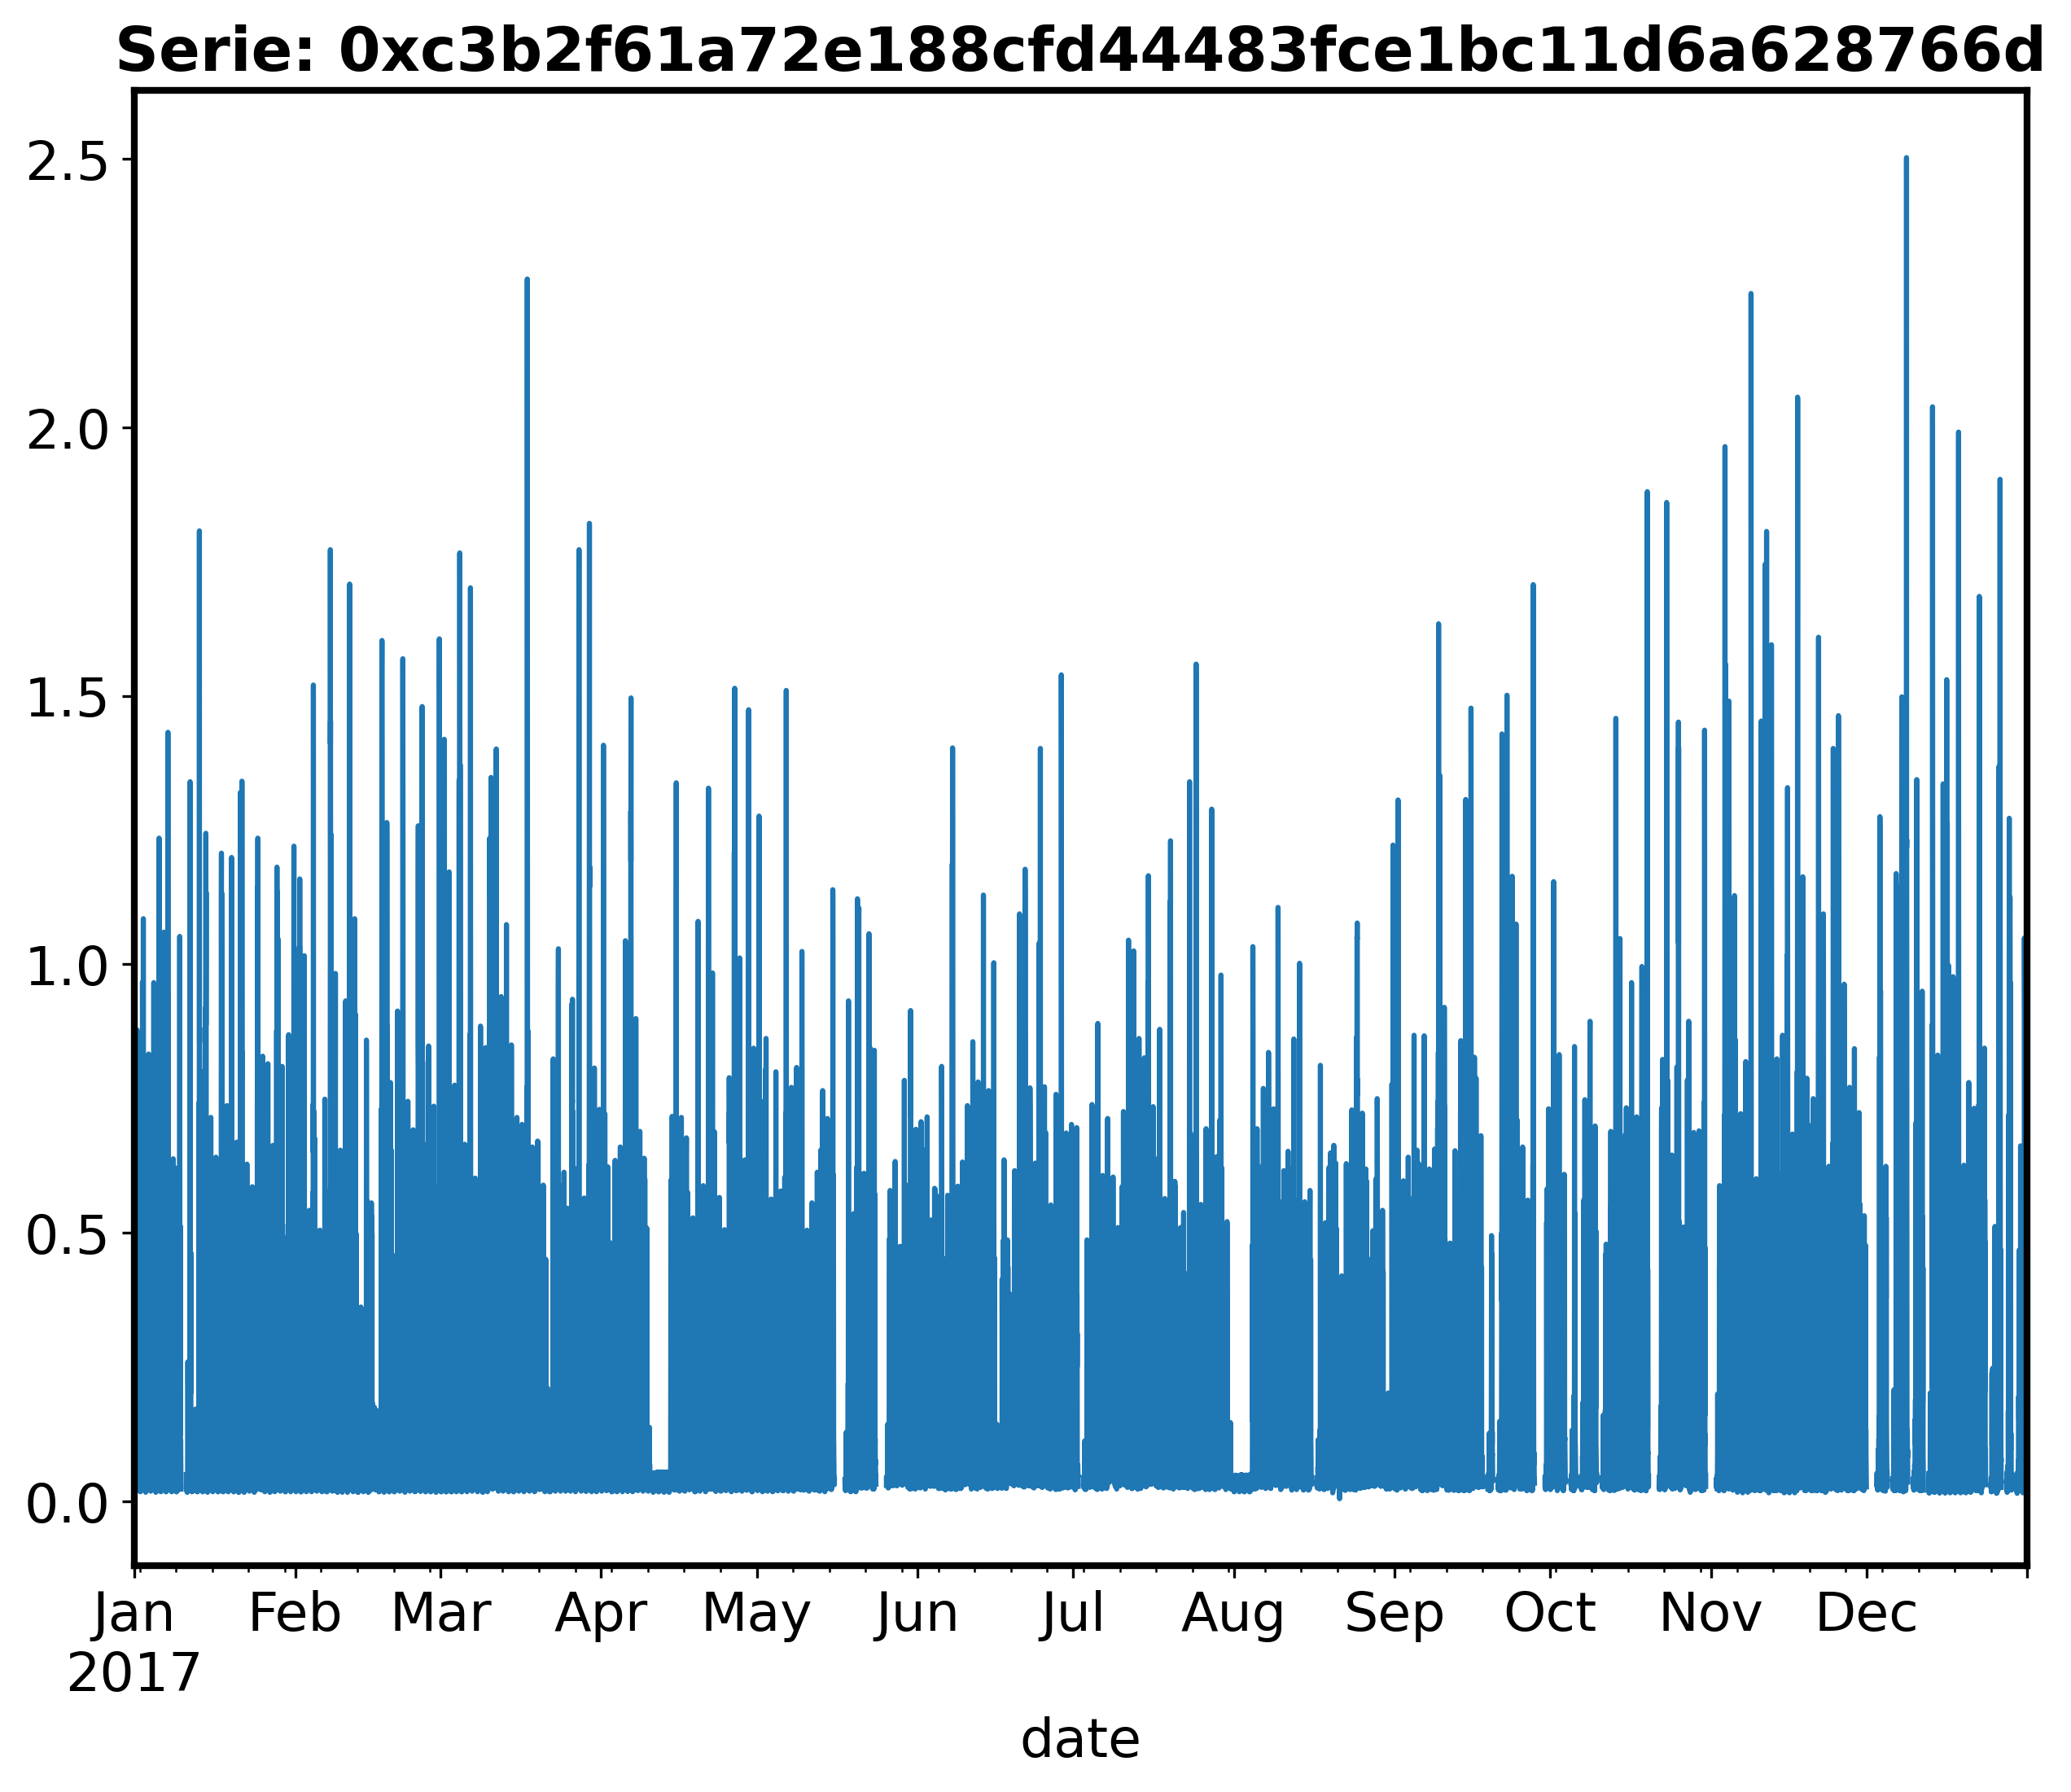
\includegraphics[width=1\linewidth]{Serie0xc3b2f61a72e188cfd44483fce1bc11d6a628766d.png}
		\caption{Serie $ 3 $}
	\end{subfigure}
	\caption{The three selected series. }
\end{figure}

\begin{table}
  \centering
  \begin{tabular}{@{}l|llr@{}} \toprule
  	\textbf{Characteristic}	& \textbf{Serie $ 1 $} & \textbf{Serie $ 2 $} & \textbf{Serie $ 3 $}\\\midrule
    Mean daily consumption [kWh]& $ 14.55 $&$ 3.17 $  & $ 6.58 $ \\
    Standard deviation daily consumption [kWh] &$ 3.21 $ & $ 0.99 $& $ 2.57 $ \\
    Median daily consumption [kWh] & $ 14.09 $ & $ 2.96 $& $ 5.88 $ \\
    Maximum daily consumption [kWh] & $ 30.08 $ & $ 6.60 $ &  $ 17.15 $   \\
    Minimum daily consumption [kWh]& $ 7.51 $ & $ 1.83 $ &  $ 1.50 $   \\
    Total missing days (consumption) & $ 4 $ &$ 25 $ & $ 26 $\\
    Days in validation set (November)&  $ 30 $ & $ 29 $  & $ 29 $ \\
    Days in Test set (December) & $ 31 $  $ 23 $  &    $ 31 $  & $ 23 $ \\
    Days in training set (Rest)&   $ 300 $  &  $ 288 $   &  $ 287 $\\
    Mean average temperature [$\degree C$]& $ 10.37 $  &  $ 10.61 $  & $ 10.22 $ \\
    Standard deviation average temperature [$\degree C$]& $ 5.09 $  & $ 5.20 $   & $ 5.01 $ \\
    Median average temperature [$\degree C$] &  $ 10.46 $ &  $ 10.61 $  & $ 10.35 $ \\
    Maximum average temperature [$\degree C$] & $ 23.99 $  & $ 24.51 $   & $ 22.95 $ \\ 
    Minimum average temperature [$\degree C$] & $ -1.07 $  &  $ -1.28 $  & $ -1.42 $ \\
    Missing average temperature days &  $ 0 $ & $ 0 $  & $ 0 $  \\ 
    Amount of holidays in $ 2017 $ & $ 8 $  &  $ 8 $  & $ 8 $ \\
  \end{tabular}
  \caption{summarizing characteristics about the selected series.}
  \label{tab:ok}
\end{table}

The three time series are divided in a training, validation and test set. As validation and test set are respectively the months November and December chosen. Because in this chapter the time series are not aggregated to a single signal as was the case in Section \ref{s:Analysis} the min-max normalization can be used. The missing values in the consumption are substituted by making use of following baseline models in order: ``previous week'' model, ``previous day'' model and the mean model. When a baseline can't make a forecast because the data is not available, a next baseline model is used. Similar, the missing values of the temperature are substituted by first looking at the temperature yesterday, then tomorrow and as last the mean temperature.\\

The simulations that are done in the chapter are performed on a virtual machine through the Microsoft Azure service.
Table \ref{tab:CPU} shows the different features of the hired machine. 
\begin{table}[hb]
	\centering
	\begin{tabular}{|p{2cm}|p{2cm}|p{2cm}|p{2cm}|}\hline
		\textbf{Name}	& \textbf{Logical cores} & \textbf{RAM (GB)} & \textbf{Storage (GB)}\\\hline
		F4s v2& $ 4 $&$ 8 $  & $ 32 $ \\\hline
	\end{tabular}
	\caption{Specifications of the virtual machine.}
	\label{tab:CPU}
\end{table}


\section{Baseline models}\label{s:Baseline models}
As earlier discussed, the baseline models are characterised by a low calculation load during training and therefore serve as a baseline to compare more complex models with. The different baseline models tried are listed as follows:
\begin{itemize}
	\item Model 1: ``closest day forecast''
	\item Model 2: ``1 day ago forecast''
	\item Model 3: ``7 days ago forecast''
	\item Model 4: ``Mean forecast''
	\item Model 5: ``MAPE forecast''
\end{itemize} 

For all the models listed here, the training set for the forecast of the next day are all the days before this day of the year $ 2017 $. These models can therefore be categorized as ``lazy models'' because they only do work when they are asked a query. In contrast, the models discussed in Section \ref{s:Neural network models} generalize the training data without knowing the actual query. The 24 hour predictions made by all $ 5 $ are done all at once, which means that predictions done for an earlier hour of the day, are not taken into account.\\

\textbf{Model 1: ``closest day forecast''}\\
This model looks for the most similar day in the training set based on following metrics to make a prediction:

\begin{itemize}
	\item Holiday
	\item Day of the week
	\item Difference average temperature
\end{itemize}
 
 It is assumed that the average temperature of the next day is available, which is a very plausible assumption.

The models listed above don't make use of a validation set. Therefore all 

- all in once forecast
- no val

\textbf{Model1: ``closest day forecast''}\\


- show all four plots --> MAPE was not possible because of the division by zero

The metrics used to evaluate the predictions performance of the base line are $ RMSE $ (Eq. \ref{eq:RMSE}), $ NRMSE $ (Eq. \ref{eq:NRMSE}), $ MAE $ (Eq. \ref{eq:MAE}), $ MSE $ (Eq. \ref{eq:MSE}) and $ MAPE $ (Eq. \ref{eq:MAPE}).

\begin{equation}\label{eq:MSE}
	MSE = \frac{\sum_{t=1}^{N}(\hat{y}_t-y_t)^2}{N}
\end{equation}

\begin{equation}\label{eq:MAPE}
	MAPE = \frac{\sum_{t=1}^{N}\abs{\hat{y}_t-y_t}/y_t}{N}
\end{equation}




Base model
Can't plot the Mape figure because sometimes the real value is equal to zero. 99 time-series have sometimes a zero consumption during half an hour.
The different base models can behave quite different on the different time-series. Sometimes the closest day works better than previous week or day and sometimes works much worse. Doesn't make a lot of sense to average the base models over all the possible time-series. 

Experiment of forecasting three time-series

Looking at the bar plots

Mean forecast behaves best  for the three time series and for all the different metrics.
%MAPE_forecast behaves often second best:
%--> serie 0xc3b: RMSE, NRMS, MSE, MAE,
%-->serie 0x78a: no times second best
%-->serie 0x1e: MAE, 
%
%In serie 0xc3b the closest, day and week perform similar and worse.
%In serie 0x78a all behave similar bad except for the mean technique
%In serie 0x1e the closest day forecast performs much better than the prev day and week method. This method is again very serie dependent.
In this serie the prev week and day behave worse than the other techniques. Similar day and MAPE work here clearly better.

Three other techniques which is best, depends a lot about which time serie is forecasted. 
When look at mse --> the amount that mean performs better gets bigger. Indication that mean is better in predicting also when occuring peak,
Because this is what the mse penalizing more severly than the other methods. Verify this with the individual plots in the tekst.
This is possibly due to the square. The MAE gives a more all similar behaviour than the other metrics.

Looking at the day plots
The previous day and week and similar forecast have typically much peaks but shifted.
The MAPE and the mean forecasts follow more the trends.

Important that when do predictions --> only look at the values in December where there is a day forecast for all the different techniques. This is in order to make a fair prediction. 
serie 0x78a--> all 31 days
serie 0x1e--> 12 days
serie 0xc3b --> 12 days
Disadvantage of previous day, previous week and similar week is that there can be not a forecast available! 
This is mostly the case for prev day and prev week. This issue is not occuring for the mean and MAPE options. 

Experiment to look at all the time series
All the 261 time-series are set to be equally important. In every time-serie a comparison with the performance of the worst technique is made.
The worst forecasting technique is set to have a value one and the rest of the techniques get a value how much better they perform than the worst signal. Which technique performs worst, depends on every time-serie.
If the mean performance is better for one technique than the other this means that the to expect performance for a random time-serie for one technique is better than the other technique. This is because this techniques behaved  more often or more proportional better than the worst technique in comparison of the other technique over all the time series. 


for one technique the performance in comparison with the worst technique 
Was on average better than the other technique. 


\section{Neural network models}\label{s:Neural network models}
- predicting each time one sample
- discuss the inputs to the models
Typical variables used in a forecasting model are: past electricity consumption loads, weather information, calendar information and error-correction terms \cite{loadforecastingmoor}.
\subsection{LSTM}
- model
- as metric for the model during training --> chosen for mse.


\subsection{GRU}

\subsection{Parameter search} \ref{s:Parameter search}
Multithreading is used to use the full potential of the CPU listed in Table \ref{tab:CPU} and simultaneously use all the available logical cores to run different threads. 

\subsection{Temperature model}
A MLP model for developing a regresion model to forecast a temperature signal. 


\subsection{Evaluation of different designs}


\section{Conclusion}


%%% Local Variables: 
%%% mode: latex
%%% TeX-master: "thesis"
%%% End: 
